\chapter{Discussion}

In this chapter, we discuss the the insights gained from building each of the unique features of our system and the design choices that went into their development. We also look at how some of these features can be extended to support additional genomic analysis tasks. We then explore some of the limitations of our current system based on the feedback gathered from our user evaluation study and possible improvements that can be made in the future.

 \section{Design Implications}
 
\begin{itemize}
    \item \textbf{Input Files and Formats} - Genomic conservation can be detected through a wide range of tools, which means that it can be represented in a wide variety of file formats depending on the type and the level of information about conservation of gene order.
    Although some tools like Mizbee have relied on users to supply input in a standardized format, this is not a viable solution as this often means users will have to rely on a custom script to transform their analysis files into the required format. Visualization tools like SynVisio and Mizbee are part of a larger ecosystem of genomic analysis tools. So they need to offer at least partial connectivity between such tools which means outputs of most analysis systems should be directly supported in visualizations tools without the need for intermediate processing. In an effort to address this developers should consider building systems that offer support for heterogeneous data. For example, SynVisio currently supports inputs from several popular tools such as collinearity files generated by MCScanX or Orthologous files generated by Dagchainer with also partial support for MUMmer output files. 
 
    \item \textbf{Web Accessibility} - Most existing genomic visualization tools are desktop applications or packages in languages such as R, Python, or Perl, however, there has been a gradual shift towards the web in the recent years. Although desktop applications are efficient at utilizing system resources, they are limited in their accessibility as they are not often supported in all operating systems and require extensive customization from developers as they are platform dependant. Web applications, on the other hand, are platform independent and can be built once and used everywhere thus requiring less development effort. Even though web apps are limited in their processing capability, they can rely on remote servers for intensive processing, and some applications like SynVisio also rely on web workers to process data in parallel threads for more efficient data processing. This easy accessibility and low-cost maintenance of web apps coupled with support for collaborative work mean that web applications should be the first choice for developers of visualization tools in the future.
    
    \item \textbf{Multi Layout and Multi Scale Views} - 
    Genomic data can be analyzed at multiple resolutions and the visual representations vary at each level. At the genome level, visual representations are chosen to emphasize approximate positions of the conserved regions and their chromosomal identifiers. This can be useful in scenarios such as during genome assemblies when errors or breaks in chromosomes can be easily identified. However, when looking at the chromosome level, orientation of the conserved region is also highlighted and finally at the individual gene level emphasis is placed exclusively on the order of collinear genes and their exact function and location in the genome. Visual representations can also vary based on the task at hand. For example, dot plots are a popular choice for summarizing large scale datasets as they offer a compact representation of both the position and orientation of conserved regions. However, their orthogonal representation is difficult to understand, making them an unpopular choice for browsing and locating selective conserved regions in comparison to parallel plots. Other such examples are stacked parallel plots which are good at tracing collinear regions across several genomes. Thus in designing genomic visualization systems, developers should rely on a combination of visual representations or provide users the choice to switch between different representations based on the task at hand. 

    \item \textbf{Visual Navigation and Linked Views} - When exploring genomic data, visualization systems can provide users several ways to traverse the different representations at each genomic scale. However, the most intuitive way to explore such a dataset would be to start at the genome level and drill down all the way into the individual gene level. So visualizations at each level should be provided with interaction techniques to filter and zoom into a particular part of the dataset which can then be viewed in a different visualization at the next inner level. This form of tiered navigation combined with the support for revisitation at any point can help researchers in easily going back and forth between the levels and exploring a large number of scenarios without losing context. Also, a major part of analyzing genomic conservation involves comparison, and providing linked multi-views that are different representations of the same information can help users in contextualizing the conservation and better understanding it.
    
    \item \textbf{Linear vs Non Linear Representations} - Genomic data is usually linear and so the best form of representing such data would be a linear representation such as a dot plot or a parallel plot but circos style plots which are a form of non-linear representation are still quite popular in genomic visualizations as they are aesthetically pleasing and offer a compact picture. However, based on observations from our user evaluation, several users found circos plots challenging to navigate for an in-depth analysis. This is primarily due to the non linear curves in these plots than can make it difficult to identify connections between distinct groups which in this case are chromosomes ordered in a circular layout. While linear representations like parallel plots can be stacked on top of each other to represent conservation between multiple genomes, circular layouts can only handle a limited number of chromosomes in the central layer before they become difficult to comprehend due to close proximity between the chromosomes. Part of the compact nature of the circos style plot arises from its ability to stack several circular layers on top of each other to represent several tracks, however, the radial nature of this design means that tracks in the outer layers are always larger than the tracks in the inner layer. This can lead to visual bias where patterns in the outer layers are more prominent than patterns in the inner layers.
    
    \item \textbf{Adaptable Genome Scales} - Genomic data can be incredibly diverse in size and so systems visualizing such information need to automatically adapt to different scales of data instead of relying on a standard scale. Some plant genomes like wheat are extremely large (17 Gigabases) and quite dispersed due to which the genes are quite small and so when visualizing this information, SynVisio provides users 2 additional levels to magnify the dataset. Similarly, when visualizing extremely small genomes such as viral genomes (30 Kilobases) the system automatically loads up the data in the smallest possible resolution directly at the gene level as shown in Figure \ref{fig:ch_7_viral} which compares similarity between two coronavirus strains that led to global pandemics. This disparity in genome sizes can also be an issue when comparing multiple genomes with a vast difference in their sizes. In such scenarios, the visualization system should provide users an option to have different scales for each of the genomes instead of relying on a single normalized scale among the genomes. 
\end{itemize}

\begin{figure}[h]
  \centering
  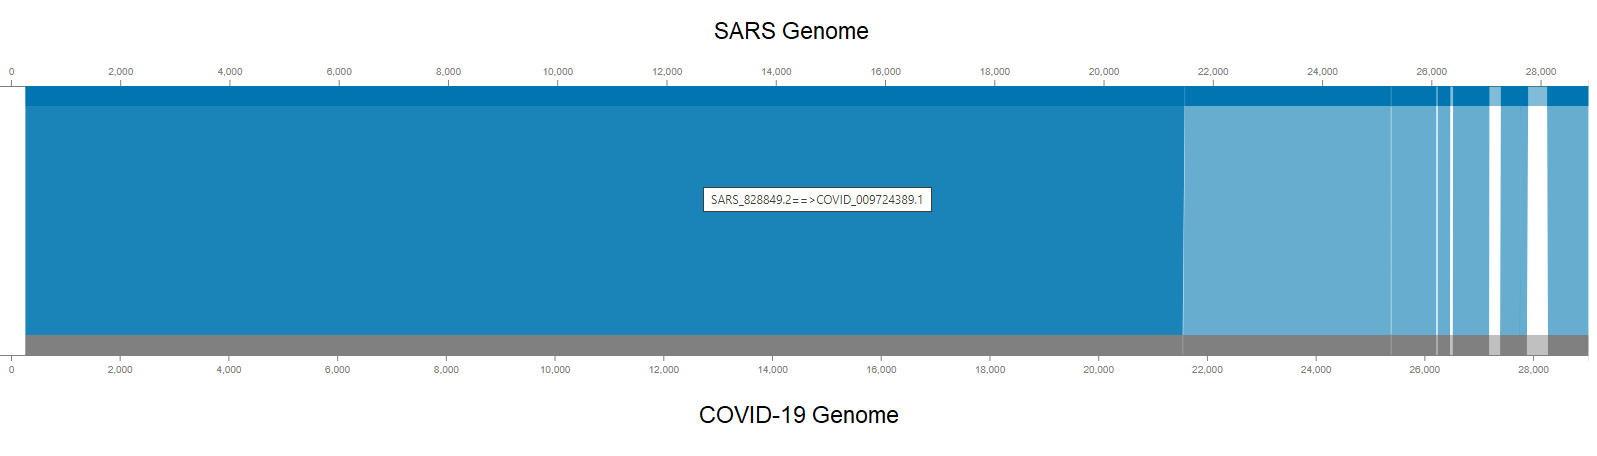
\includegraphics[width=1\linewidth]{images/ch_7_viral.PNG}
  \captionof{figure}{Similarity between genomes of the SARS Virus (2003 pandemic) and the COVID-19 Virus (2019-2020 pandemic) with the RNA responsible for a single protein highlighted in a darker shade.}
  \label{fig:ch_7_viral}
\end{figure}


 \section{Limitations and Future Work}
 
 Although SynVisio was designed to handle a wide variety of scenarios, there are still certain issues with our system that can be improved through additional changes in the future. 
 
 \begin{itemize}
    \item The first and major limitation of our system lies in the dependence on an external tool (MCScanX, DAGChainer or Mummer) to detect conserved regions. This was mentioned as a bottleneck by several of our users in analyzing their datasets. But the complexity involved in detecting similarity between two given sequences and running a collinearity detection software cannot be achieved through the existing web system as it is computation intensive. A possible way in which this can be solved in the future is by setting up a dedicated remote server that can accept sequences uploaded by users to perform synteny detection on the cloud and then send the results back to the web system to be visualized. This would also give users greater flexibility in changing the different parameters involved in detecting conserved regions such as the E-value  to look at more distant matches.    
    
    \item SynVisio is currently opinionated in determining the visual scale of the genome. Genome scales are calculated based on the available screen width and the size of the genome in base pairs and every chromosome is normalized accordingly. But users are given the option to override the normalization and have independent scales for each genome when comparing multiple genomes. This can lead to confusion when two genomes are stacked parallel to each other, and both stretch to fill the available width causing users to lose context of the size of the genomes. To address this confusion in future, we can provide information in the form of tracks or scales indicating the size of the genome in Kilo-bases or Mega-bases.
    
    \item SynVisio automatically sorts chromosomes alphanumerically in each genome to determine their layout. These chromosomes are then presented from left to right and oriented in the same direction. However, in some cases, this layout can cause the ribbons connecting conserved regions to excessively cross each other, making it difficult to understand the relation between the two genomes. In such scenarios, it would be helpful if users are provided an option to declutter the layout by reordering the chromosomes or reversing the orientation of each chromosome. This can be achieved in the future by developing a dedicated layout editor that lets users manual drag chromosomes around and reverse them if needed to create a more organized layout.
    
    \item Visualizing syteny in stacked parallel plots is an excellent way to trace conserved regions across multiple genomes. However, researchers are often also interested in understanding the evolutionary relationship between a given set of genomes along with an overview of the conserved regions between them. Evolutionary relationships among genomes are commonly represented as phylogenetic trees evolving from shared ancestors. Combining such a representation along with the existing parallel plots between genomes would be a significant improvement to SynVisio and offer researchers an easy way to analyze novel datasets such as the pan-genomes of different species.
    
    \item Although SynVisio lets users explore genomic data from the genome level all the way down to the individual genome level, it cannot show the actual nucleotide or the protein sequence alignment within every gene. This limitation arises due to the large size of FASTA files which cannot be loaded directly onto the Web interface. However, presenting this information can help researchers in understanding the extent of similarity in the gene alignment and gain additional information about the function of the gene and the protein it codes for. For most annotated genes, several online databases exist that curate this information and present it in a easily accessible manner such as genomeDB and NCBI. In future, we would like to link every gene in the gene level directly to their entries in preexisting databases, such that clicking on any gene would automatically open up the FASTA entry along with information about that gene in a new tab of the browser.    


\end{itemize}
 
